
\documentclass[12pt, a4paper, oneside, romanian]{teza-upb}
\setcounter{secnumdepth}{3}
\setcounter{tocdepth}{3}
\usepackage{babel}
\usepackage{graphicx}
\usepackage{adjustbox}
\usepackage{caption}
\usepackage{subcaption}
\usepackage{babel}
\usepackage{color}
\usepackage{graphicx}
\usepackage{ragged2e}
\usepackage{multirow}
\usepackage{amsmath}
\usepackage{mathtools}
\usepackage{enumitem}
\usepackage{float}
\usepackage{fontenc}
\usepackage{afterpage}
\usepackage{pdfpages}
\usepackage[
  bookmarks,
  bookmarksopen=true,
  pdftitle={Licenta},
  linktocpage]{hyperref}
\usepackage{url}

\singlespacing

%%%%%%%%%%%%%%%%%%%%%%%%%%%%%%%%%%%%%%%%%%%%%%%%%%%%%%%%cod colorat
\usepackage{listings}
\usepackage{color}
 
\definecolor{codegreen}{rgb}{0,0.6,0}
\definecolor{codegray}{rgb}{0.5,0.5,0.5}
\definecolor{codepurple}{rgb}{0.58,0,0.82}
\definecolor{backcolour}{rgb}{0.95,0.95,0.92
}
\DeclarePairedDelimiter\ceil{\lceil}{\rceil}

\newcommand\blankpage{%
    \null
    \thispagestyle{empty}%\
    \addtocounter{page}{-1}
    \newpage}

\lstdefinestyle{mystyle}{
	language=Matlab,
 %   backgroundcolor=\color{backcolour},   
    commentstyle=\color{codegreen},
    keywordstyle=\color{blue},
    numberstyle=\tiny\color{codegray},
    stringstyle=\color{codepurple},
	basicstyle=\ttfamily\scriptsize,
    breakatwhitespace=false,         
    breaklines=true,                 
    captionpos=b,                    
    keepspaces=true,                 
    numbers=left,                    
    numbersep=5pt,                  
    showspaces=false,                
    showstringspaces=false,
    showtabs=false,                  
    tabsize=2
}
 
\lstset{style=mystyle}
%%%%%%%%%%%%%%%%%%%%%%%%%%%%%%%%%%%%%%%%%%%%%%%

\begin{document}

\author{Stancovici Marian}

\title{Analiza imaginilor cu fund de ochi pentru ajutor în diagnosticul retinopatiei diabetice}


\facultatea{Facultatea de Electronică, Telecomunicații și Tehnologia Informației}
\tiplucrare{dizertație}
\domeniu{Calculatoare si Tehnologia Informatiei}
\catedra{Telecomunicații}
\campus{Leu}
\program{Ingineria Informaţiei}
\titlulobtinut{Master}
\director{Conf. dr. ing. Laura Maria FLOREA}

\submissionmonth{Iunie}
\submissionyear{2026}

\beforepreface

\newpage
\mbox{}
\newpage

\listoffigures

\listoftables

\newpage
\mbox{}
\newpage

\abbreviations{
  SOTA = State of the Art\\
  Deep DRiD = Deep Diabetic Retinopathy Image Dataset\\
  UoA-DR = University of Auckland Diabetic Retinopathy\\
}
%\preface{}
\afterpreface

\afterpage{\blankpage}

\chapter*{Introducere}

\section*{Contextul și motivația lucrării}

\ \ \ \ Retinopatia diabetică reprezintă o provocare majoră de sănătate publică, fiind principala cauză a
orbirii prevenibile în rândul populației active. Creșterea continuă a numărului de pacienți cu diabet
generează o presiune imensă asupra sistemelor medicale, depășind adesea capacitatea de screening a
specialiștilor. Deoarece afecțiunea poate evolua asimptomatic în fazele inițiale, identificarea pacienților
la risc este critică înainte ca leziunile retiniene să devină ireversibile, subliniind necesitatea unor soluții
de monitorizare scalabile și eficiente.
\bigskip

Complexitatea diagnosticării este dată de necesitatea unei clasificări precise, conform
standardelor internaționale care împart boala în cinci clase de severitate \cite{6_wang2021deep}, \cite{11_shakibania2024dual}. Procesul impune
medicului să distingă între stadiile incipiente, marcate doar de microanevrisme discrete \cite{13_staal2004ridge}, și formele
avansate, caracterizate de hemoragii și neovascularizație. Această granularitate a diagnosticului este
dificilă de menținut constant în programele de screening în masă, unde oboseala și subiectivitatea
factorului uman pot duce la erori de clasificare cu impact direct asupra deciziilor terapeutice.
\bigskip

Pentru a depăși aceste limitări, domeniul imagisticii medicale a adoptat rapid soluțiile bazate pe
inteligență artificială. Trecerea de la metodele clasice de procesare a imaginii \cite{2_sopharak2009automatic} la algoritmii de învățare
profundă (Deep Learning) a marcat un punct de inflexiune, validat clinic prin studii extensive \cite{3_gulshan2016development}. Rețelele
neurale convoluționale au eliminat necesitatea definisrii manuale a regulilor vizuale \cite{4_pratt2016convolutional}, având capacitatea
de a învăța autonom trăsături complexe direct din datele brute \cite{9_chetoui2020explainable} și de a identifica corelații subtile între
texturi și patologie.
\bigskip

Evoluția recentă a acestor tehnologii a permis tranziția de la modele experimentale simple la
arhitecturi robuste \cite{7_huang2022rtnet}, capabile să opereze în condiții clinice reale. Cercetarea actuală s-a distanțat de
clasificarea binară elementară, concentrându-se pe sisteme care pot gestiona variabilitatea imaginilor
provenite din diverse surse prin tehnici de adaptare la domeniu \cite{8_zhang2022multi}. Algoritmii moderni demonstrează o
reziliență crescută la artefacte și zgomot vizual, oferind o consistență a diagnosticului care rivalizează cu
expertiza umană \cite{9_chetoui2020explainable}, \cite{10_jabbar2022transfer}.

\section*{Obiectivele lucrării}

\ \ \ \ Scopul lucrării de față este de a folosi algoritmi de vedere computerizată bazați pe rețele convoluționale adânci pentru a crea o metodă de detectare
si clasificare a retinopatiei diabetice. Metoda se va testa pe seturi de date publice. Implementarea se va face în Python folosind biblioteci specifice.
\bigskip

Aceasta urmărește atingerea următoarelor obiective:

\begin{itemize}
  \item Analizarea metodelor deja propuse în literatura de specialitate pentru detecția și clasificarea automată a retinopatiei diabetice folosind 
  imagini cu fund de ochi.

  \item Căutarea seturilor de date publice ce conțin imagini cu fund de ochi și adnotări pentru clasificarea retinopatiei diabetice.

  \item Analizarea seturilor de date găsite.

  \item Propunerea unei metode bazate pe învățare profundă pentru detecția și clasificarea retinopatiei diabetice.

  \item Analizarea performanței pentru metoda propusă în diverse cazuri de antrenare/testare
\end{itemize}

\section*{Structura lucrării}

Lucrarea de față este structurată în mai multe capitole, fiecare din ele abordând un subiect esențial din proiect:

\begin{itemize}
  \item Capitolul 1: Introducere
        \begin{itemize}[label={}]
          \item În acest capitol se prezintă contextul și motivația lucrării, cât și cum se propune să se redacteze si să se structureze, menționând aplicabilitatea acesteia in lumea reală.
        \end{itemize}

  \item Capitolul 2: Fundamente teoretice - context medical și tehnic
        \begin{itemize}[label={}]
          \item[] Acest capitol va oferi o privire de ansamblu asupra retinopatiei diabetice, explicând cauzele, simptomele și stadiile acestei afecțiuni, precum și importanța detecției și clasificării automate a acesteia. De asemenea, se vor introduce conceptele de bază ale învățării profunde și ale rețelelor neuronale convoluționale, care vor fi utilizate în dezvoltarea metodei propuse.
        \end{itemize}

  \item Capitolul 3: Metode existente pentru detecția automată a retinopatiei diabetice
        \begin{itemize}[label={}]
          \item[] Acest capitol va oferi o analiză detaliată a metodelor existente pentru detecția și clasificarea retinopatiei diabetice, evidențiind avantajele și limitările acestora, precum și modul în care acestea au evoluat în timp.
        \end{itemize}

  \item Capitolul 4: Metodologie și implementare
        \begin{itemize}[label={}]
          \item[] Acest capitol va detalia metodologia și implementarea propusă pentru detecția și clasificarea retinopatiei diabetice, explicând arhitectura rețelei neuronale utilizate, procesul de antrenare și optimizare, precum și modul în care aceasta se diferențiază de metodele existente.
        \end{itemize}

  \item Capitolul 5: Metoda propusă
        \begin{itemize}[label={}]
          \item[] Acest capitol va detalia metoda propusă pentru detecția și clasificarea retinopatiei diabetice, explicând arhitectura rețelei neuronale utilizate, procesul de antrenare și optimizare, precum și modul în care aceasta se diferențiază de metodele existente.
        \end{itemize}

  \item Capitolul 6: Rezultate experimentale și discuții
        \begin{itemize}[label={}]
          \item[] Acest capitol va prezenta rezultatele obținute în urma testării metodei propuse pe seturile de date alese, comparând performanța acesteia cu alte metode existente și discutând avantajele și limitările sale.
        \end{itemize}

  \item Capitolul 7: Concluzii
        \begin{itemize}[label={}]
          \item[] Acest capitol va sintetiza concluziile generale ale lucrării, evidențiind contribuțiile aduse și impactul potențial al metodei propuse în domeniul detecției automate a retinopatiei diabetice.
        \end{itemize}
\end{itemize}

\newpage
\mbox{}
\newpage


\chapter{Fundamente teoretice - context medical și tehnic}

\section{Diabetul zaharat și complicațiile sale oculare}

\section{Anatomia ochiului și retina}

\section{Retinopatia diabetică — definiție, stadii de evoluție și simptome}

\section{Imagistica de fund de ochi ("fundus photography")}

\section{Diagnosticul clinic — procesul actual și limitările sale}


\chapter{Metode existente pentru detecția automată a retinopatiei diabetice}

\section{Analiza seturilor de date disponibile}

\ \ \ \ Performanța și capacitatea de generalizare a modelelor de învățare profundă sunt intrinsec
dependente de calitatea, volumul și diversitatea datelor utilizate în procesul de antrenare. În contextul
oftalmologiei computaționale, disponibilitatea bazelor de date publice a permis tranziția de la metodele
clasice de procesare a imaginii la arhitecturi neuronale complexe, oferind un teren comun pentru
evaluarea obiectivă a algoritmilor.

\begin{itemize}
  \item \textbf{Seturi de referință pentru clasificarea globală (“Grading”)}
  
        \begin{itemize}
            \item \textbf{EyePACS} (Kaggle Diabetic Retinopathy Detection) \cite{3_gulshan2016development}, \cite{9_chetoui2020explainable} rămâne cea mai 
                  vastă resursă publică disponibilă, conținând aproximativ 88.702 de imagini. Importanța sa strategică constă în eterogenitatea
                  extremă a imaginilor (variații de expunere, focalizare, artefacte), fiind critic pentru antrenarea unor
                  rețele backbone robuste capabile să gestioneze fenomenul de “domain shift” \cite{8_zhang2022multi} și să generalizeze pe
                  imagini de calitate slabă

            \item \textbf{APTOS 2019} Blindness Detection \cite{9_chetoui2020explainable} reprezintă standardul modern de calitate. Colectat de Aravind Eye
                  Hospital, acest set de 3.662 de imagini este utilizat frecvent în literatura recentă pentru “fine-tuning”,
                  oferind o vizibilitate superioară a detaliilor retiniene comparativ cu seturile mai vechi

            \item \textbf{MESSIDOR-2} \cite{9_chetoui2020explainable} este considerat în prezent „Benchmark-ul de Aur” pentru testarea algoritmilor.
                  Extinzând setul original Messidor la 1.748 de imagini, acesta se distinge prin consistența diagnostică și
                  este utilizat ca domeniu țintă (Target Domain) în studiile de adaptare \cite{8_zhang2022multi} și pentru validarea sistemelor
                  explicabile (XAI) \cite{9_chetoui2020explainable}, oferind o metrică fidelă a performanței reale pe date curate.

            \item \textbf{DeepDRiD} \cite{14_liu2022deepdrid} aduce o inovație necesară prin structurarea
                  celor 2.000 de imagini în perechi binoculare și includerea notelor de calitate, simulând fluxul de triaj
                  clinic.

            \item \textbf{UoA-DR} \cite{9_chetoui2020explainable} este o resursă istorică (~200 imagini), utilizată
                  complementar în studiile comparative pentru a asigura diversitatea demografică a validării.
        \end{itemize}

  \item \textbf{Seturi specializate pentru segmentarea leziunilor și analiza detaliată}

        \begin{itemize}
          \item 
        \end{itemize}

  \item 
\end{itemize}

\section{Module dedicate}
\subsection{Timer}
\subsection{UART}
\subsection{SPI}
\subsection{GPIO}
\subsection{AXI RAM}
\section{Modulul de top și instanțierea SoC-ului}
\section{Logica de test și integrarea EDT}

\chapter{Metodologie și implementare}
\section{Sinteza circuitului}
\subsection{introducerea logicii DFT (lanuturi de SCAN)}
\subsection{Importarea librariilor si optimizare}
\section{Generarea vectorilor de test pentru defecte STUCK-AT și TRANSITION}
\subsection{Cazul fără EDT (fastscan)}
\subsection{Cazul cu EDT (variante cu 30, 40, 50, 60 de lanturi de SCAN)}
\section{Regenerarea EDT-ului și crearea netlist-ului pentru modulul de top}
\section{Simularea vectorilor de test și generarea testbench-ului}
\section{Etapa de diagnoză}

\chapter{Rezultate și discuții (ATPG)}
\section{Criterii de performanță ale sistemului pentru diferite variante de test (non-EDT vs EDT-30/40/50/60 chains)}
\ \ \ \ În acest capitol se vor sintetiza toate informațiile discutate la capitolele anterioare, atât despre sinteză cât și pe partea de generare de vectori de test pentru toate cazurile, și se vor analiza și discuta rezultatele obținute, făcându-se o comparație obiectivă.
Următoarea figură prezintă toate rezultatele comprimate într-un tabel cu metrici de performanță.

\begin{figure}[H]
  \centering
  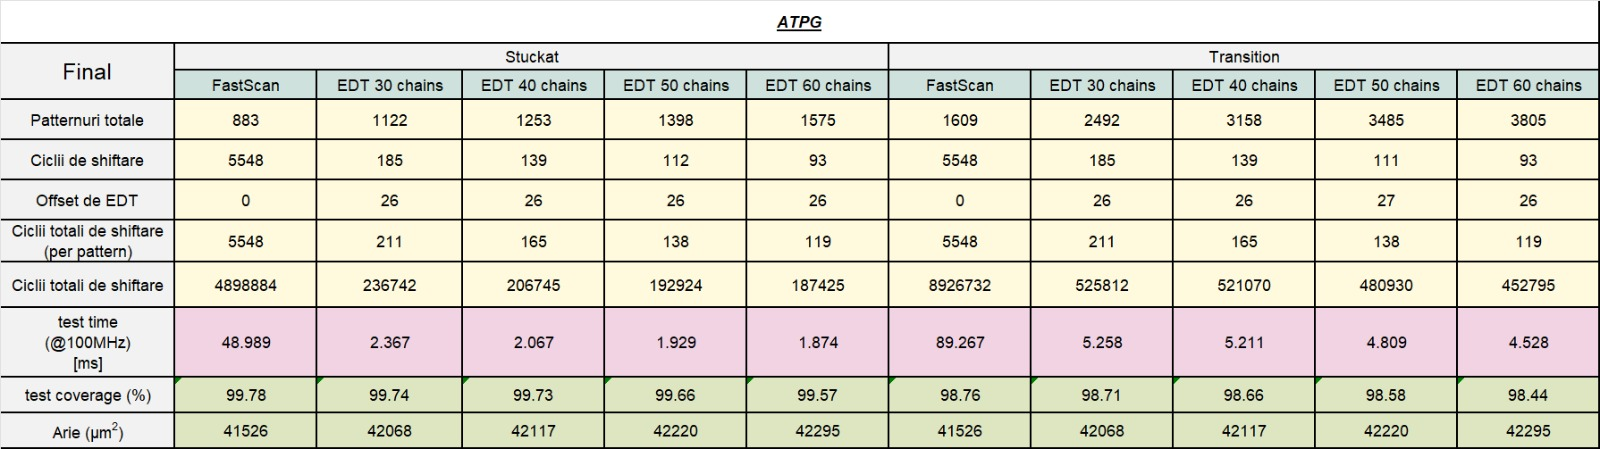
\includegraphics[width=1\columnwidth]{Figuri/Overview_ATPG.jpeg}
  \caption{Tabelul cu metrici de evaluare pentru generarea patternurilor de test}
  \label{fig: Overview_ATPG}
\end{figure}

Rezultatele s-au obținut pe urma simulărilor de generare de vectori de test pentru ATPG normal, respectiv pentru ATPG folosindu-se EDT cu 30,40,50 sau 60 de lanțuri de scan, aceste simulări realizându-se pentru a detecta defecte de tip stuck-at și transition.

În continuare se va lua pe rând fiecare metrică și se va explica utilitatea acesteia și rezultatele ei.

\subsection{Patternuri de test}
\ \ \ \ După cum se poate observa, în cazul ATPG-ului normal s-au generat 883 de vectori de test (acest număr nu se poate anticipa), în timp ce, integrând modulul de EDT, crește considerabil numărul de vectori de test generați. Acest lucru se întâmplă din următoarele cauze:
\begin{itemize}

  \item EDT-ul, așa cum se specifică și în denumirea acestuia, se concentrează pe metode deterministice de generare de vectori de test care vizează defecte și modele de defecte specifice. Acestea sunt mai eficiente decât metodele aleatoare, dar tind să genereze un număr mai mare de vectori de test.
  \item EDT-ul este conceput să detecteze defecte greu de detectat cu medote de ATPG tradiționale, realizând acest lucru prin adăugarea de logică de test suplimentară în circuit pentru a crește observabilitatea și controlabilitatea nodurilor interne. Acest lucru necesită mai multe patternuri de test pentru un test-coverage cât mai mare.
  \item Diferența în numărul de lanțuri de scan.

        În cazul fără EDT există un singur lanț de scan, în timp ce, adăugând modulul de EDT, se pot configura mai multe lanțuri de scan prin care datele se deplasează în paralel, ajungând la mai multe patternuri de test.

\end{itemize}

De asemenea, numărul de vectori de test se mărește și în cazul în care se crește numărul lanțurilor de scan pentru EDT. Cu cât numărul acestora este mai mare, cu atât scade gradual lungimea fiecărui lanț de scan și numărul de flip-flopi prin care circulă datele este distribuit mai multor lanțuri, ceea ce produce efectulul descris.

Cât despre tipul de defect, există câteva motive principale de ce este nevoie de un număr mult mai mare de vectori de test pentru a detecta defecte de tip transition decât cele de tip stuck-at:
\begin{itemize}
  \item \textbf{Propagarea defectului}: Defectele de tranziție au nevoie ca vectorul de test respectiv să poată propaga efectul până într-un punct observabil din circuit fără a se pierde între timp, în comparație cu defectele stuck-at care doar blochează intrarea sau ieșirea unei porți la o valoare fixă.
  \item \textbf{Considerente de sincronizare}: Defectele transition sunt mult mai sensibile la sincronizarea tranziției semnalelor de la o valoare în alta, ceea ce conduce la mai mulți vectori de test pentru a putea capta timpii necesari detectării defectului.
\end{itemize}

\subsection{Ciclii de shiftare}
\ \ \ \ Un ciclu de shiftare reprezintă o deplasare a datelor cu o poziție în lanțul de scan corespunzător. Cum în cazul ATPG normal este prezent un singur lanț de scan, numărul cicliilor este egal cu dimensiunea lanțului respectiv deoarece datele circulă prin toți flip-flopii de scan înainte să fie măsurați la ieșire.

În restul cazurilor (EDT), numărul total de celule de scan se împarte la numărul scan chain-urilor și se obține numărul de ciclii de ceas pentru un lanț de scan, datele circulând în paralel.
Exemplu pentru EDT cu 30 de lanțuri de scan:
\[ \text{ciclii shiftare} = \frac{\text{număr total de celule de scan}}{\text{număr lanțuri de scan}} = \frac{5548}{30} = 185 \]

Tipul de defect nu afectează acest număr deoarece logica de testare din interiorul modulului principal nu se modifică.

\subsection{EDT Offset}
\ \ \ \ Din perspectiva ATE-ului, design-ul prezintă un singur lanț de scan care circulă prin intrarea edt\_channels\_in înainte să intre în decompresor.

Acest aspect se întamplă doar în cazul EDT-ului, iar fiecare pattern necesită un număr de ciclii de shiftare adiționali care se adună la numărul de patternuri din fiecare lanț calculat la punctul anterior.

Acesti ciclii adiționali provin din modul de funcționare și structura EDT-ului, mai exact din \cite{TKompressManual}:
\begin{itemize}
  \item ciclii de initializare
  \item biții de mascare (dacă se folosește o tehnologie specializată numită Xpress)
  \item biți de low-power (când se folosește un decompresor de putere scăzută)
  \item biții de pipeline definiți de utilizator
\end{itemize}

Numărul de ciclii de inițializare se poate calcula cu ajutorul următoarei formule \cite{TKompressManual} :
\[ \text{număr ciclii de inițializare} =  \ceil{\frac{\text{dimensiunea decompresorului}}{\text{numărul de canale}}}\], unde fracția se rotunjește la valoarea sa superioară.
De exemplu, dacă avem un design în care decompresorul are dimensiunea de 32 de biți și există 6 canale de scan, iar numărul de celule de scan din fiecare lanț este 870, atunci este nevoie de 6 ciclii de inițializare. Fiecare lanț având 870 de celule și fiecare vector comprimat având nevoie de 6 ciclii de inițializare, rezultă că este nevoie de 876 de deplasări per pattern (nefolosind ceilalți biți).

Acest număr se adună în continuare celorlalte elemente din lista de mai sus, rezultând astfel numărul total de ciclii de shiftare suplimentari:
\[\text{ciclii suplimentari} = \text{ciclii de inițializare} + \text{biți de mascare} +\text{biți de low-power} + \text{biți de pipeline}\]
În cazul nostru, din rapoartele de simulare reiese că exista 26 de ciclii suplimentari, care se vor aduna la lungimea lanțului de scan, rezultând numărul total de ciclii de shiftare.

\subsection{Ciclii totali de shiftare (per pattern)}
\ \ \ \ Așa cum s-a specificat anterior, numărul de ciclii totali de shiftare reprezintă suma dintre numărul de ciclii propriu-zis și offset-ul de EDT, în cazul ATPG-ului obișnuit acesta este 0.

\subsection{Ciclii totali de shiftare}
\ \ \ \ Folosind numărul de ciclii de shift per pattern și numărul total de patternuri de test, putem calcula numărul total de ciclii de shift pentru întreg modulul cu ajutorul următoarei formule:
\[\textbf{\text{ciclii totali de shift} = \text{ciclii de shift per pattern}}\times \textbf{\text{număr de patternuri}}\]

Cu ajutorul acestei metrici se poate determina dimensiunea memoriei necesare pentru efectuarea simulărilor de generare de patternuri.

\subsection{Timp de testare}
\ \ \ \ Cum fiecare element din lanțurile de scan reprezintă flip-flipi de scan care sunt celule secvențiale de memorie, acestea functionează în mod sincron cu ceasul sistemului.
Prin urmare, folosindu-ne de frecvența sistemului putem calcula timpul necesar deplasării datelor prin lanțurile de scan folosind toate patternurile generate.
Acesta se calculează cu formula:
\[ \text{timp de testare} = \text{număr total de ciclii} \times \frac{1}{\text{frecvența ceasului de sistem}} \]

În cazul de față frecvența ceasului de sistem este 100MHz, ceea ce înseamnă că o perioadă de ceas are 0.01 $\mu$s, adică 10 ns.
De exemplu, pentru cazul cu 30 lanțuri de scan, avem 236.742 ciclii totali, ceea ce înseamnă că timpul total de testare este 2.367.420 ns, aproximativ 2,36 secunde.

De asemenea, având în vedere că datele circulă în paralel prin lanțuri, timpul de testare este mult mai mic în cazul utilizării EDT-ului în comparație cu ATPG normal (20 ori mai mic).

\subsection{Test Coverage}
\ \ \ \ În contextul design-for-testing (DFT), noțiunea de "test-coverage" se referă la măsura în care un set de teste aplicate unui sistem sau circuit electronic acoperă sau verifică toate părțile și funcționalitățile prevăzute.
Acoperirea testelor este o metrică importantă a calității procesului de testare și al nivelului de încredere pe care ne putem baza ca sa știm dacă produsul nu mai prezintă defecte dupa ce a fost testat.
\vspace{0.4cm}

După cum se poate observa din tabel, cu cât numărul de lanțuri de test este mai mare, cu atât test-coverage-ul este mai mic (putem spune că sunt mărimi invers proporționale), deoarece circuitul devine mai puțin controlabil din punct de vedere al testării.
Cu alte cuvinte, un raport de compresie mai mare duce la mărirea compresiei pentru fiecare pattern de test, dar de asemenea crește și posibilitatea generării de patternuri care nu pot fi comprimate și care duc în final la un test-coverage mai mic.

\subsection{Arie}
\ \ \ \ Deși nu este o metrică atat de importantă pentru testare precum test-coverage-ul, am vrut să evidențiez 2 aspecte:
\begin{itemize}
  \item Logica EDT adaugă o porțiune foarte mică de hardware suplimentar în circuit.

        În acest caz având un modul cu doar 64000 de porți logice, logica suplimentară introdusă este de aproximativ 1\%, însă pentru un chip în curs de testare care prezintă milioane de porți, logica introdusă pentru EDT ajunge undeva la 0,35\% din arie, ceea ce este o adiție infimă în comparație cu timpul de test câștigat.

  \item Cu cât creștem numărul de lanțuri de scan, cu atât crește aria folosită, însă foarte puțin în comparație cu aria totală, coverage-ul scăzând și el deoarece circuitul este din ce în ce mai greu de testat.

\end{itemize}

\chapter{Concluzii}

\section{Direcții viitoare de cercetare și dezvoltare}
\ \ \ \ Cu toate ca această lucrare reprezintă un pas important în implementarea și testarea circuitelor digitale pentru detectarea defectelor de fabricație folosind vectori de test generați automat, există multiple direcții viitoare de cercetare și dezvoltare care pot îmbunătăți și extinde rezultatele obținute.
Acestea includ următoarele, dar nu se limitează la acestea:
\begin{itemize}
  \item \textbf{\textit{Optimizarea performanței sistemului de testare}}: Un aspect esențial care poate fi explorat este optimizarea performanței sistemului de testare. În mod specific, se pot studia metode avansate de reducere a timpului de testare fără a compromite acuratețea și acoperirea testelor. Algoritmi noi și tehnici de optimizare a scan chain-urilor și a vectorilor de test pot contribui semnificativ la îmbunătățirea eficienței procesului de testare.

  \item \textbf{\textit{Integrarea noilor tehnologii de testare}}: Pe măsură ce tehnologia avansează, noi metode și instrumente de testare devin disponibile. Integrarea acestor tehnologii, precum tehnici avansate de Built-In Self-Test (BIST) sau utilizarea inteligenței artificiale pentru generarea și analiza vectorilor de test, poate îmbunătăți semnificativ capacitatea de detectare a defectelor și eficiența procesului de testare.

  \item \textbf{\textit{Extinderea scalabilității}}: Un alt domeniu de cercetare este extinderea scalabilității sistemului de testare pentru circuite mai complexe și mari. Explorarea modului în care tehnologiile actuale de SCAN și EDT pot fi adaptate și extinse pentru system-on-chips (SoC) de dimensiuni mai mari și cu complexitate sporită poate duce la îmbunătățiri importante în detectarea defectelor.

  \item \textbf{\textit{Dezvoltarea de metode de testare pentru noi tipuri de defecte}}: În timp ce lucrarea de față se concentrează pe detectarea defectelor de tip STUCKAT și TRANSITION, există și alte tipuri de defecte care pot afecta performanța circuitelor digitale. Cercetarea și dezvoltarea unor metode de testare pentru detectarea defectelor de tip delay, crosstalk și defecte intermitente poate asigura o acoperire mai completă și o fiabilitate crescută a circuitelor testate.

  \item \textbf{\textit{Implementarea și validarea în cazuri practice}}: O direcție importantă de dezvoltare este aplicarea și validarea metodologiilor propuse în contexte industriale reale. Colaborarea cu industria semiconductorilor pentru implementarea soluțiilor dezvoltate în cadrul unor proiecte pilot poate oferi feedback valoros și poate ajuta la rafinarea tehnicilor de testare.

  \item \textbf{\textit{Automatizarea procesului de diagnoză}}: Deși lucrarea a abordat deja etapa de diagnoză, există loc pentru automatizarea completă a acestui proces. Dezvoltarea unor instrumente de diagnoză automată, care pot identifica rapid și precis locația defectelor în circuit, ar contribui semnificativ la reducerea timpului de depanare și la îmbunătățirea eficienței generale a procesului de testare.

  \item \textbf{\textit{Studii comparative asupra metodelor de testare și posibilitatea combinării acestora}}: Realizarea unor studii comparative între diferitele tehnologii și metode de testare disponibile poate oferi o înțelegere mai profundă a avantajelor și dezavantajelor fiecărei abordări. Aceste studii pot ghida alegerea metodologiilor optime pentru diferite tipuri de circuite și aplicații.

        De asemenea, se poate aborda în viitor o posibilă combinare a acestor metode pentru o automatizare și o eficientizare mai puternică, extrăgând punctele forte din fiecare metodă de testare.
\end{itemize}

Deci, deși s-au atins obiective importante în domeniul detectării defectelor de fabricație în circuitele digitale, există multiple direcții viitoare de cercetare și dezvoltare care pot contribui la avansarea cunoștințelor și tehnologiilor în acest domeniu. Explorarea acestor direcții poate duce la sisteme de testare mai eficiente, fiabile și scalabile, asigurând astfel calitatea și performanța superioară a circuitelor digitale.


\section{Contribuții principale si concluzii}
\ \ \ \ Lucrarea de față, intitulată "Detectia defectelor de fabricație într-un circuit digital cu ajutorul vectorilor de test generați automat", a avut ca scop implementarea unui set de teste pentru un circuit digital, pentru depistarea defectelor de fabricație (DFT). Circuitul digital, descris in limbaj Verilog, a constat dintr-un SoC bazat pe tehnologie RISC-V, cu module dedicate de Timer, UART, SPI și periferice GPIO. În acest capitol se vor sintetiza concluziile principale obținute în urma cercetării și implementării efectuate.
\vspace{0.4cm}

În cadrul acestei lucrări am utilizat tehnologii complexe de testare precum tehnologia SCAN (introducerea lanțurilor de scan în circuit + transformarea flip-flopilor în celule de scan), ATPG (generarea automata a vectorilor de test cu ajutorul constrângerilor), DFT (concept care reunește noțiunile de SCAN, ATPG, EDT) și EDT (compresia vectorilor de test pentru îmbunatățirea performanțelor).
Fiecare din aceste tehnologii a prezentat un rol esențial în îmbunătățirea detectării defectelor și optimizarea procesului de testare.

Introducerea logicii de scan în circuit, generarea vectorilor (patternurilor) de test, compresia acestora, procesul de simulare și diagnoză, pentru defecte de tip STUCKAT și TRANSITION au reprezentat exemple și aspecte esențiale în asigurarea acurateții și eficienței testării.
\vspace{0.4cm}

Unul dintre principalele obiective majore ale lucrării a fost verificarea performanțelor sistemului, în special timpul de testare și test-coverage-ul utilizând diverse structuri de test folosind generarea automată de vectori de test. În acest context, s-au analizat performanțele testării modulului atât în cazul utilizării unui singur lanț de scan, cât și în cazul utilizării multiplelor lanțuri de scan cu ajutorul tehnologiei EDT.

Rezultatele au demonstrat că utilizarea EDT a redus semnificativ timpul de testare, păstrând în același timp test-coverge-ul aproape de valoarea rezultată testarii cu un singur lanț de scan, iar testele realizate cu 30, 40, 50, respectiv 60 de lanțuri de scan au arătat că este nevoie de atenție atunci când se alege acest număr, păstrând raportul dintre timpul de testare și test coverage în balanță.
\vspace{0.4cm}

Procesul de sinteză a inclus nu doar interpretarea și importarea librăriilor pentru celulele de bază ale circuitului (porți logice, bistabile etc), cât și inserarea logicii de scan în circuit. Acesta s-a realizat prin scripturi bine definite și cu ajutorul makefile-urilor pentru a păstra ordinea și automatizarea în execuția scripturilor.

S-a efectuat analiza codului sursă HDL și al librăriilor (pentru verificarea erorilor de sintaxă și semantică din codul realizat), elaborarea design-ului (transformarea acestuia într-un format inteligibil pentru tool-ul Design Compiler), compilarea design-ului (transformarea design-ului într-o reprezentare structurală), inserția logicii de scan, cât și generarea netlist-ului sintetizat gata pentru etapa de ATPG, pe care am discutat-o anterior, în care am generat vectorii de test pentru structuri de test cu și fără EDT cu ajutorul tool-ului Tessent - Mentor Graphics.
\vspace{0.4cm}

Simularea patternurilor de test folosind SimVision a permis vizualizarea semnalelor de scan (scan\_enable, scan\_mode, cât și edt\_channels\_in, edt\_channels\_out, edt\_reset și edt\_update), și a flip-flopilor de scan interconectate în lanțuri de scan (propagarea datelor în mod secvențial prin acestea).

Acest pas a fost crucial pentru a asigura că toți vectorii de test generați detectează toate defectele vizate în mod corect și într-un timp cât mai scurt.
\vspace{0.4cm}

În etapa de diagnoză, introducerea unui defect în mod intenționat în circuit a permis testarea capacității sistemului de a identifica exact poarta logică unde se regasește defectul. Aceasta s-a depistat cu succes cu o precizie și un indice de încredere de 100\%.

Această etapă a demonstrat că metodologia de testare utilizată este robustă și capabilă să localizeze cu acuratețe defectele din circuit, confirmând astfel validitatea și eficiența abordării propuse.
\vspace{0.4cm}

Lucrarea a demonstrat că utilizarea vectorilor de test generați automat și a tehnologiilor avansate de testare, precum EDT, poate îmbunătăți semnificativ detectarea defectelor de fabricație în circuitele digitale. Implementarea și testarea efectuate au arătat că abordarea propusă nu doar că reduce timpul de testare, dar și poate păstra test-coverage-ul la o valoare acceptabilă în același timp. În concluzie, metodologia aplicată în această lucrare oferă o soluție eficientă și scalabilă pentru detectarea defectelor în circuitele digitale complexe, fiind relevantă și aplicabilă în industria semiconductoarelor.

\newpage
\mbox{}
\newpage

\appendix
\bibliographystyle{unsrt}
\bibliography{referinte}

\chapter {Cod}

\lstinputlisting[language = tcl, caption = dummy\_design.dofile]{Cod/edt_ip/dummy_design.dofile}
\vspace{1cm}

\lstinputlisting[language=bash, caption = Bash Script for generating EDT]{Cod/edt_ip/my_script_gen_edt.sh}
\vspace{1cm}



\end{document}
